\hsection{Iteration, Comprehension, and Generators}%
\label{sec:iteration}%
%
In \python, iterating over the items in a sequence is a central concept.
In \cref{sec:enumOverSequences}, we learned that we can iterate over collections such as lists, tuples, dictionaries, and sets.
We can also iterate over the characters in a string in the same way.
These are all datastructures whose complete content exists in memory at any given time.
In \python, we can also iterate over sequences where the items that are constructed at the time when they are actually needed.
A good example for this is the \pythonilIdx{range} datatype.
We can iterate over all the 1'000'000'000 \pythonil{int} elements of \pythonil{range(1_000_000_000)} in a loop.
These many integers do not all exist in memory at the same time.
Instead, they are provided one-by-one as needed.
From the perspective of a programmer, we can iterate over a \pythonilIdx{range} and a \pythonilIdx{list} in exactly the same way.
Matter of fact, many objects in \python\ support iteration.

Vice versa, we can also create container datatypes from sequences of items.
For example, the datatypes \pythonilIdx{list}, \pythonilIdx{tuple}, \pythonilIdx{set}, and \pythonilIdx{dict} can also be used like functions that take a sequence of items as parameter and create in instance of the corresponding datatype.
In \cref{sec:lists:basicFunctions}, we learned that \pythonil{[1, 2, 2, 3]} creates a list with the specified contents.
Passing this list to the \pythonilIdx{set} function/datatype, i.e., writing \pythonil{set([1, 2, 2, 3])} will create the set \pythonil{\{1, 2, 3\}}.
We also learned that we modify several datastructures in place by combining them with other containers.
Invoking \pythonil{l.extend(\{1, 2, 3\})}\pythonIdx{list!extend}\pythonIdx{extend} will append the elements~\pythonil{1}, \pythonil{2}, and \pythonil{3} to a list~\pythonil{l}, for example.

\begin{figure}%
\centering%
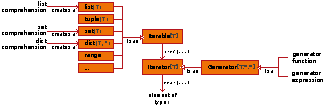
\includegraphics[width=0.96\linewidth]{\currentDir/iteration.pdf}%
\caption{The concepts of comprehension, \pythonilsIdx{Iterable}, \pythonilsIdx{Iterator}, and \pythonilsIdx{Generator} in \python.}%
\label{fig:iteration}%
\end{figure}%

Much later -- in a chapter that I have not yet written -- we learn that we also can iterate over the contents of a file.
You will very often encounter situations where you transform, process, or create sequences of data elements.
As sketched in \cref{fig:iteration}, there are many different manifestations of the concepts of \emph{iterating} over objects that are \emph{iterable} in \python.
In this chapter, we will investigate those that we did not yet already discuss in \cref{sec:enumOverSequences,sec:collections}.
%
\hsection{\texttt{Iterable}s and \texttt{Iterator}s}%
\label{sec:iterable}%
%
\begin{figure}%
\centering%
%
\subfloat[][%
Manually iterating over a \pythonilIdx{list}.%
\label{fig:iterateOverListAndRange:list}%
]{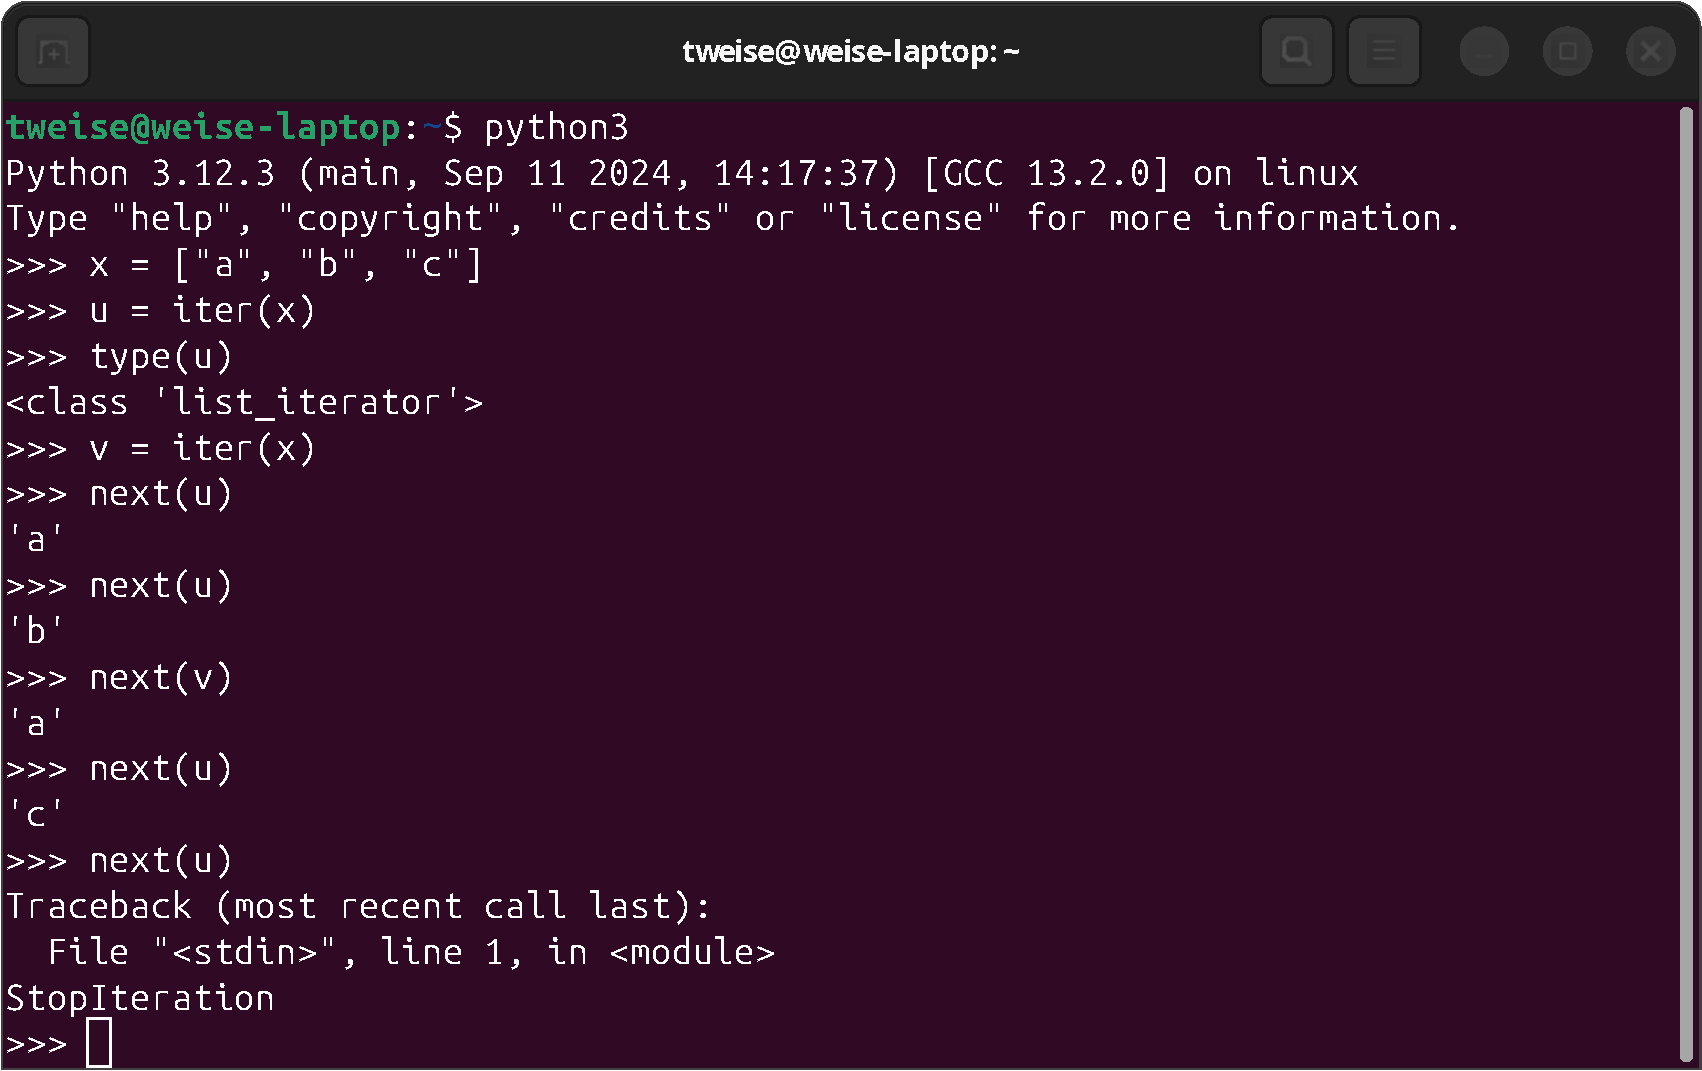
\includegraphics[width=0.7\linewidth]{\currentDir/listIterConsole}}%
%
\\[12pt]%
%
\subfloat[][%
Manually iterating over a \pythonilIdx{range}.%
\label{fig:iterateOverListAndRange:range}%
]{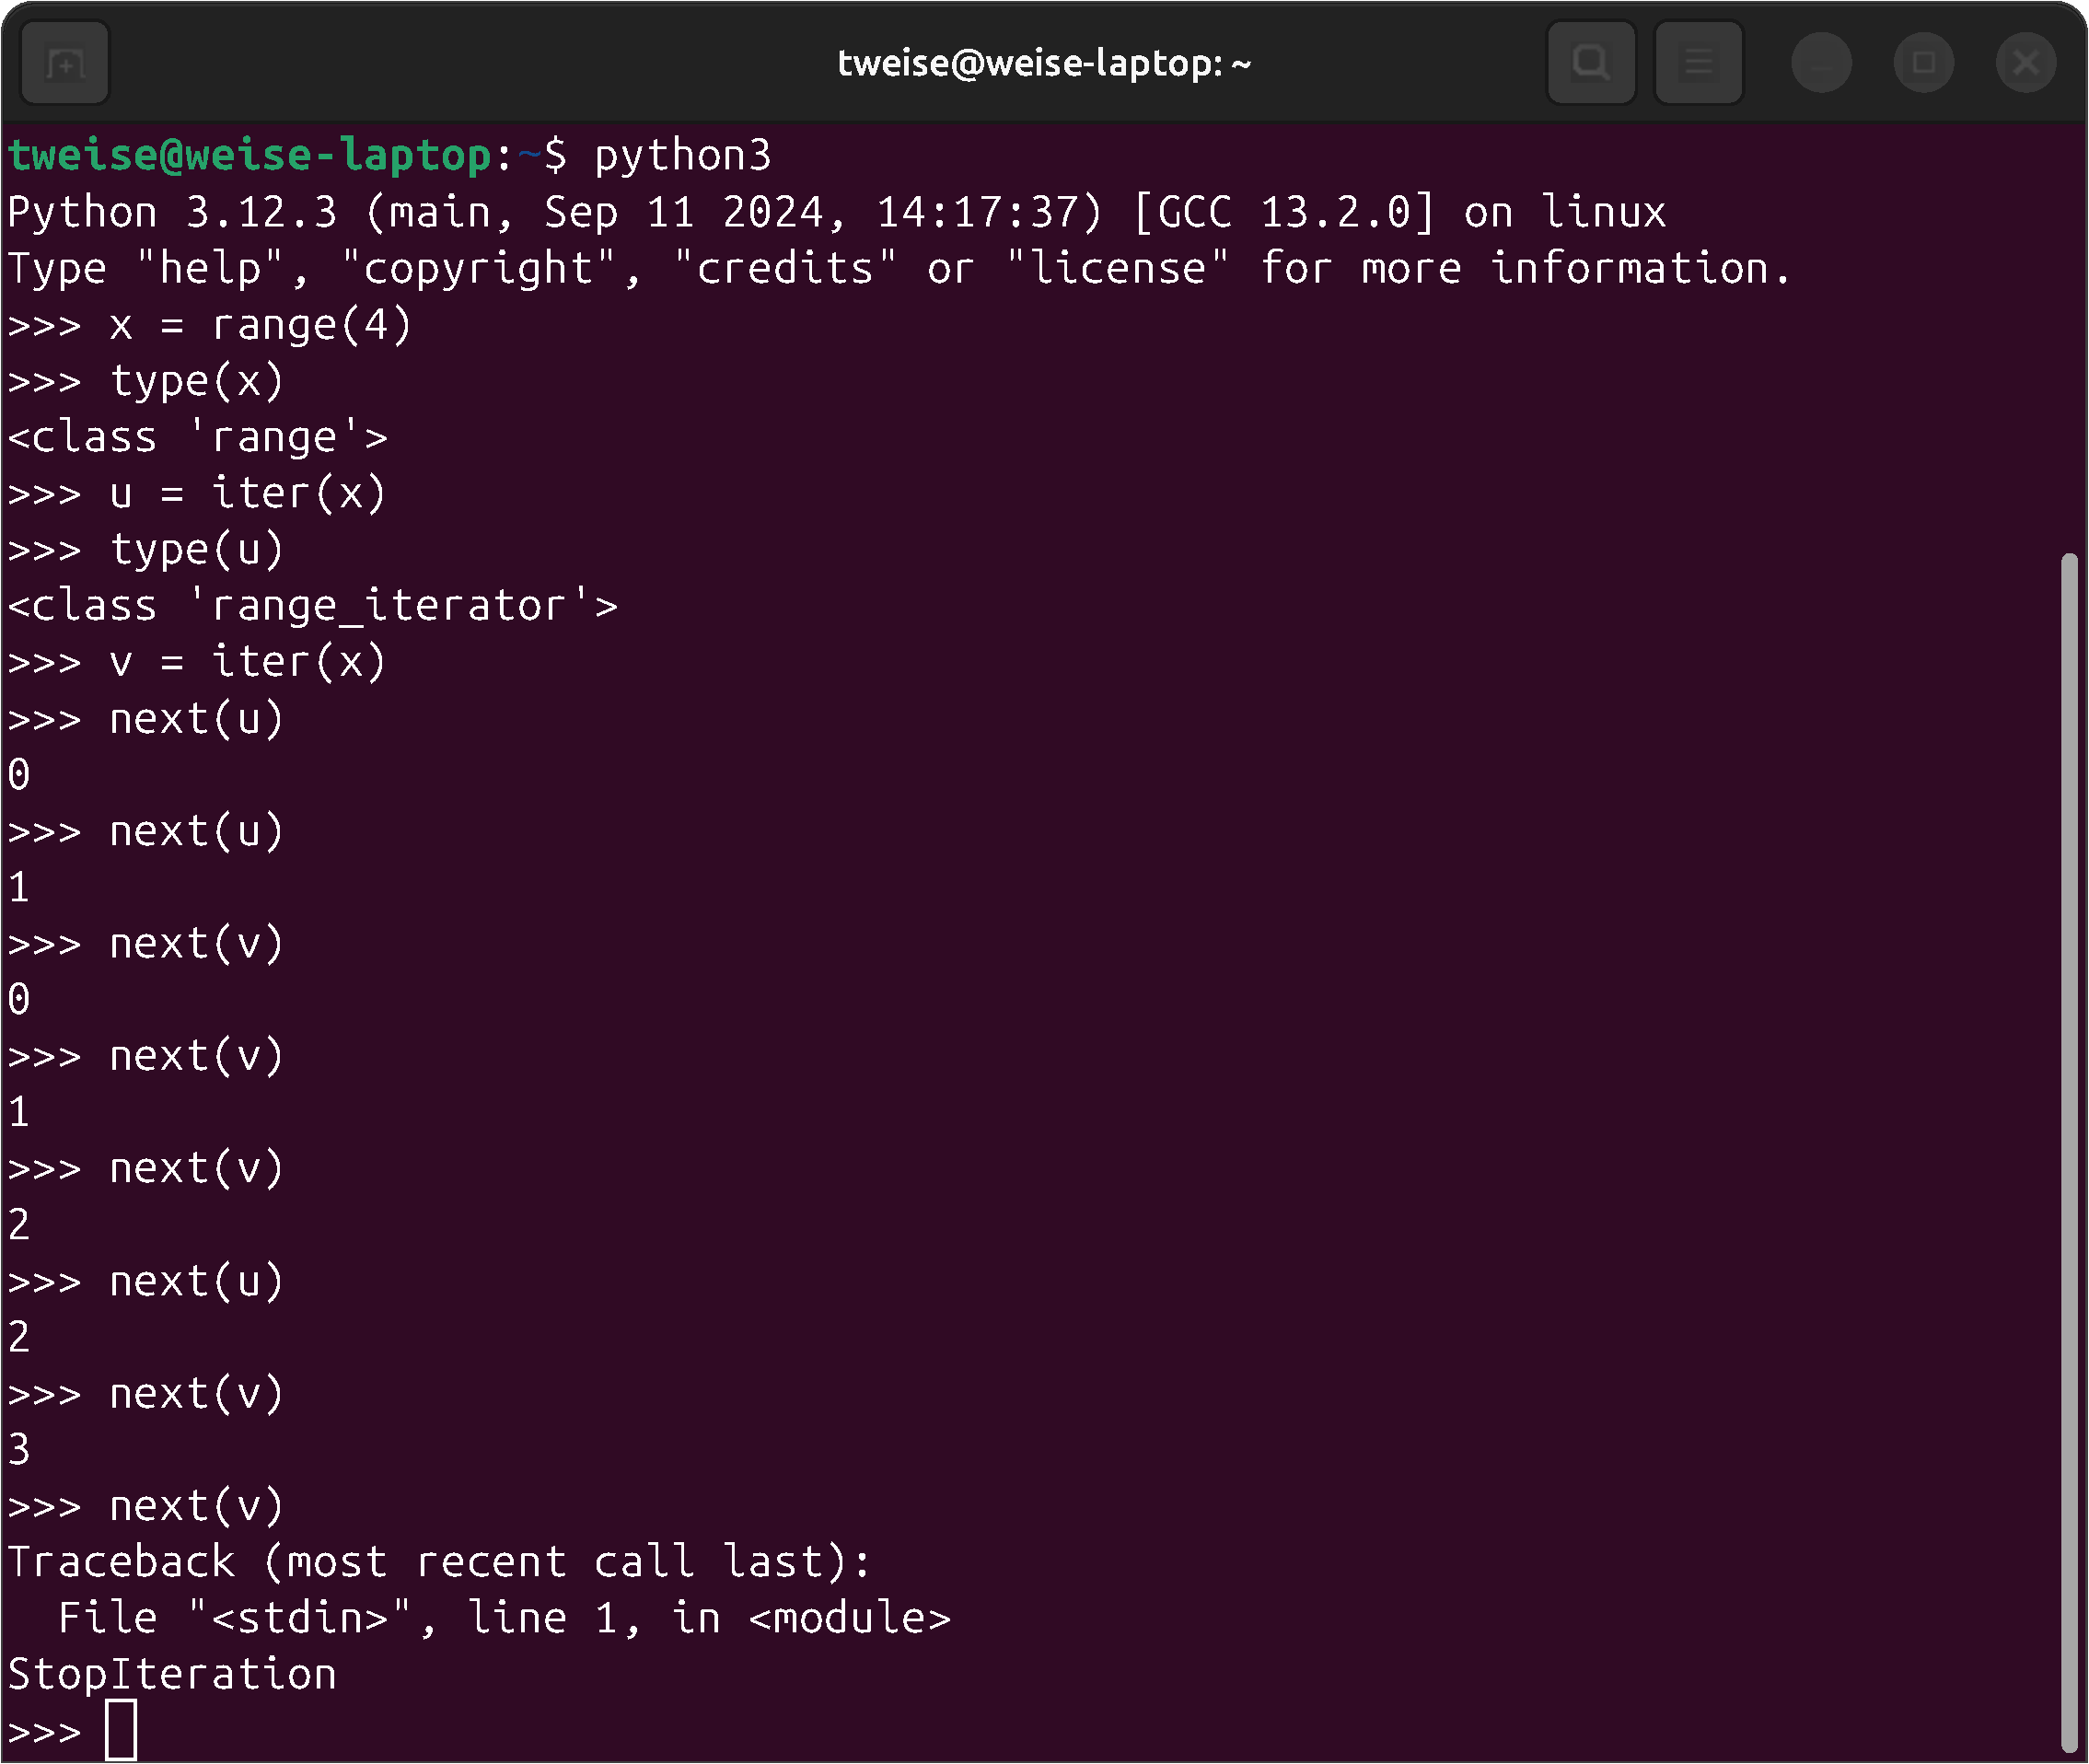
\includegraphics[width=0.7\linewidth]{\currentDir/rangeIterConsole}}%
%
%
\caption{Manually iterating over a \pythonilIdx{list} and a \pythonilIdx{range} in the \python~console.}%
\label{fig:iterateOverListAndRange}%
\end{figure}%
%
\begin{sloppypar}%
Any object that allows us to access its elements one-by-one, i.e., \emph{iteratively} is an instance of \pythonilIdx{typing.Iterable}\pythonIdx{Iterable}.
The actual iteration over the contents is then done by an \pythonilIdx{typing.Iterator}\pythonIdx{Iterator}.
This distinction is necessary because we want to allow some objects to be iterated over multiple times.%
\end{sloppypar}%
%
Let's say you have the list \pythonil{x = ["a", "b", "c"]}, as in \cref{fig:iterateOverListAndRange:list}.
We can use this list~\pythonil{x} in a \pythonil{for xi in x}-kind of loop arbitrarily often.
\pythonil{x} is an instance of \pythonilIdx{list} and every list is also an~\pythonilIdx{Iterable}\pythonIdx{typing.Iterable}.
Every time we do loop over \pythonil{x}, an \pythonilIdx{Iterator} instance is created internally by (doing something like) invoking~\pythonil{y = iter(x)}\pythonIdx{iter}.
In principle, this \pythonilIdx{Iterator} object only has to remember its current position in the list, allowing us to query the next item by invoking~\pythonil{next(y)}\pythonIdx{next}.
The \pythonilIdx{for}-loop basically does this internally.
However, we can also do it \inQuotes{by hand.}
In \cref{fig:iterateOverListAndRange:list}, we perform \pythonil{u = iter(x)} and \pythonil{v = iter(x)}.
This creates two independent \pythonilsIdx{Iterator}, which we can use to step over the list separately.
Invoking \pythonil{next(u)}\pythonIdx{next} will yield the first element of the list~\pythonil{x}, namely~\pythonil{"a"}.
Calling \pythonil{next(u)}\pythonIdx{next} again gives us the second element, that is~\pythonil{"b"}.
If we now call \pythonil{next(v)}\pythonIdx{next}, i.e., apply~\pythonilIdx{next} to the second, independent \pythonilIdx{Iterator}, we again obtain the first element~(\pythonil{"a"}).

This shows us why there is a distinction between \pythonilIdx{Iterable} and \pythonilIdx{Iterator}.
The former is the object that holds or can generate the data sequence.
The latter marks one independent iteration over that sequence.

The third invocation of \pythonil{next(u)}\pythonIdx{next} gives us~\pythonil{"c"}, the third and last element of~\pythonil{x}.
If we now call \pythonil{next(u)}\pythonIdx{next} a fourth time, something interesting happens:
A \pythonilIdx{StopIteration} is raised\pythonIdx{raise}.
This is not an error in the strict sense.
This instead is how the end of an iteration sequence is signaled.
A \pythonilIdx{for}~loop will, for instance, stop when it encounters this exception.

\Cref{fig:iterateOverListAndRange:range} shows us that \pythonilsIdx{range} have the exactly same behavior as \pythonilsIdx{list} with respect to iteration.
And they should, of course, like every other object implementing the~\pythonilIdx{Iterable} functionality.
As a result, the \pythonil{for y in x}-type of loops can be applied to any \pythonilIdx{Iterable} or \pythonilIdx{Iterator} instance~\pythonil{x}.%
%
\endhsection%
%
\endhsection%
%
